\section{Gate Voltage and Charge Carrier Density}
To understand the influence of different carrier densities $n$, the gate voltage $U_\text{gate}$ is varied.
A higher $U_\text{gate}$ increases the Fermi level and thus the carrier density.
Gate voltages of $1.5V, 1V, -0.25V, -1V, -1.5V$ have been applied.
The first three gate voltages are shown in Fig. \ref{fig:differentGateVoltagesQHE}.
They show Hall plateaus and Shoubnikow-de Haas oscillations.
The Hall resistance $\rho_\text{xy}$ grows more slowly with $B$ for larger state densities.
Note that the plateaus in $\rho_\text{xy}$ remain at the same discrete values, but require higher $B$.
This can be explained by the higher Fermi level, which has more Landau levels below it.
A higher $B$ is needed to move the Landau levels above the Fermi level.
\begin{figure}[h]
    \centering
    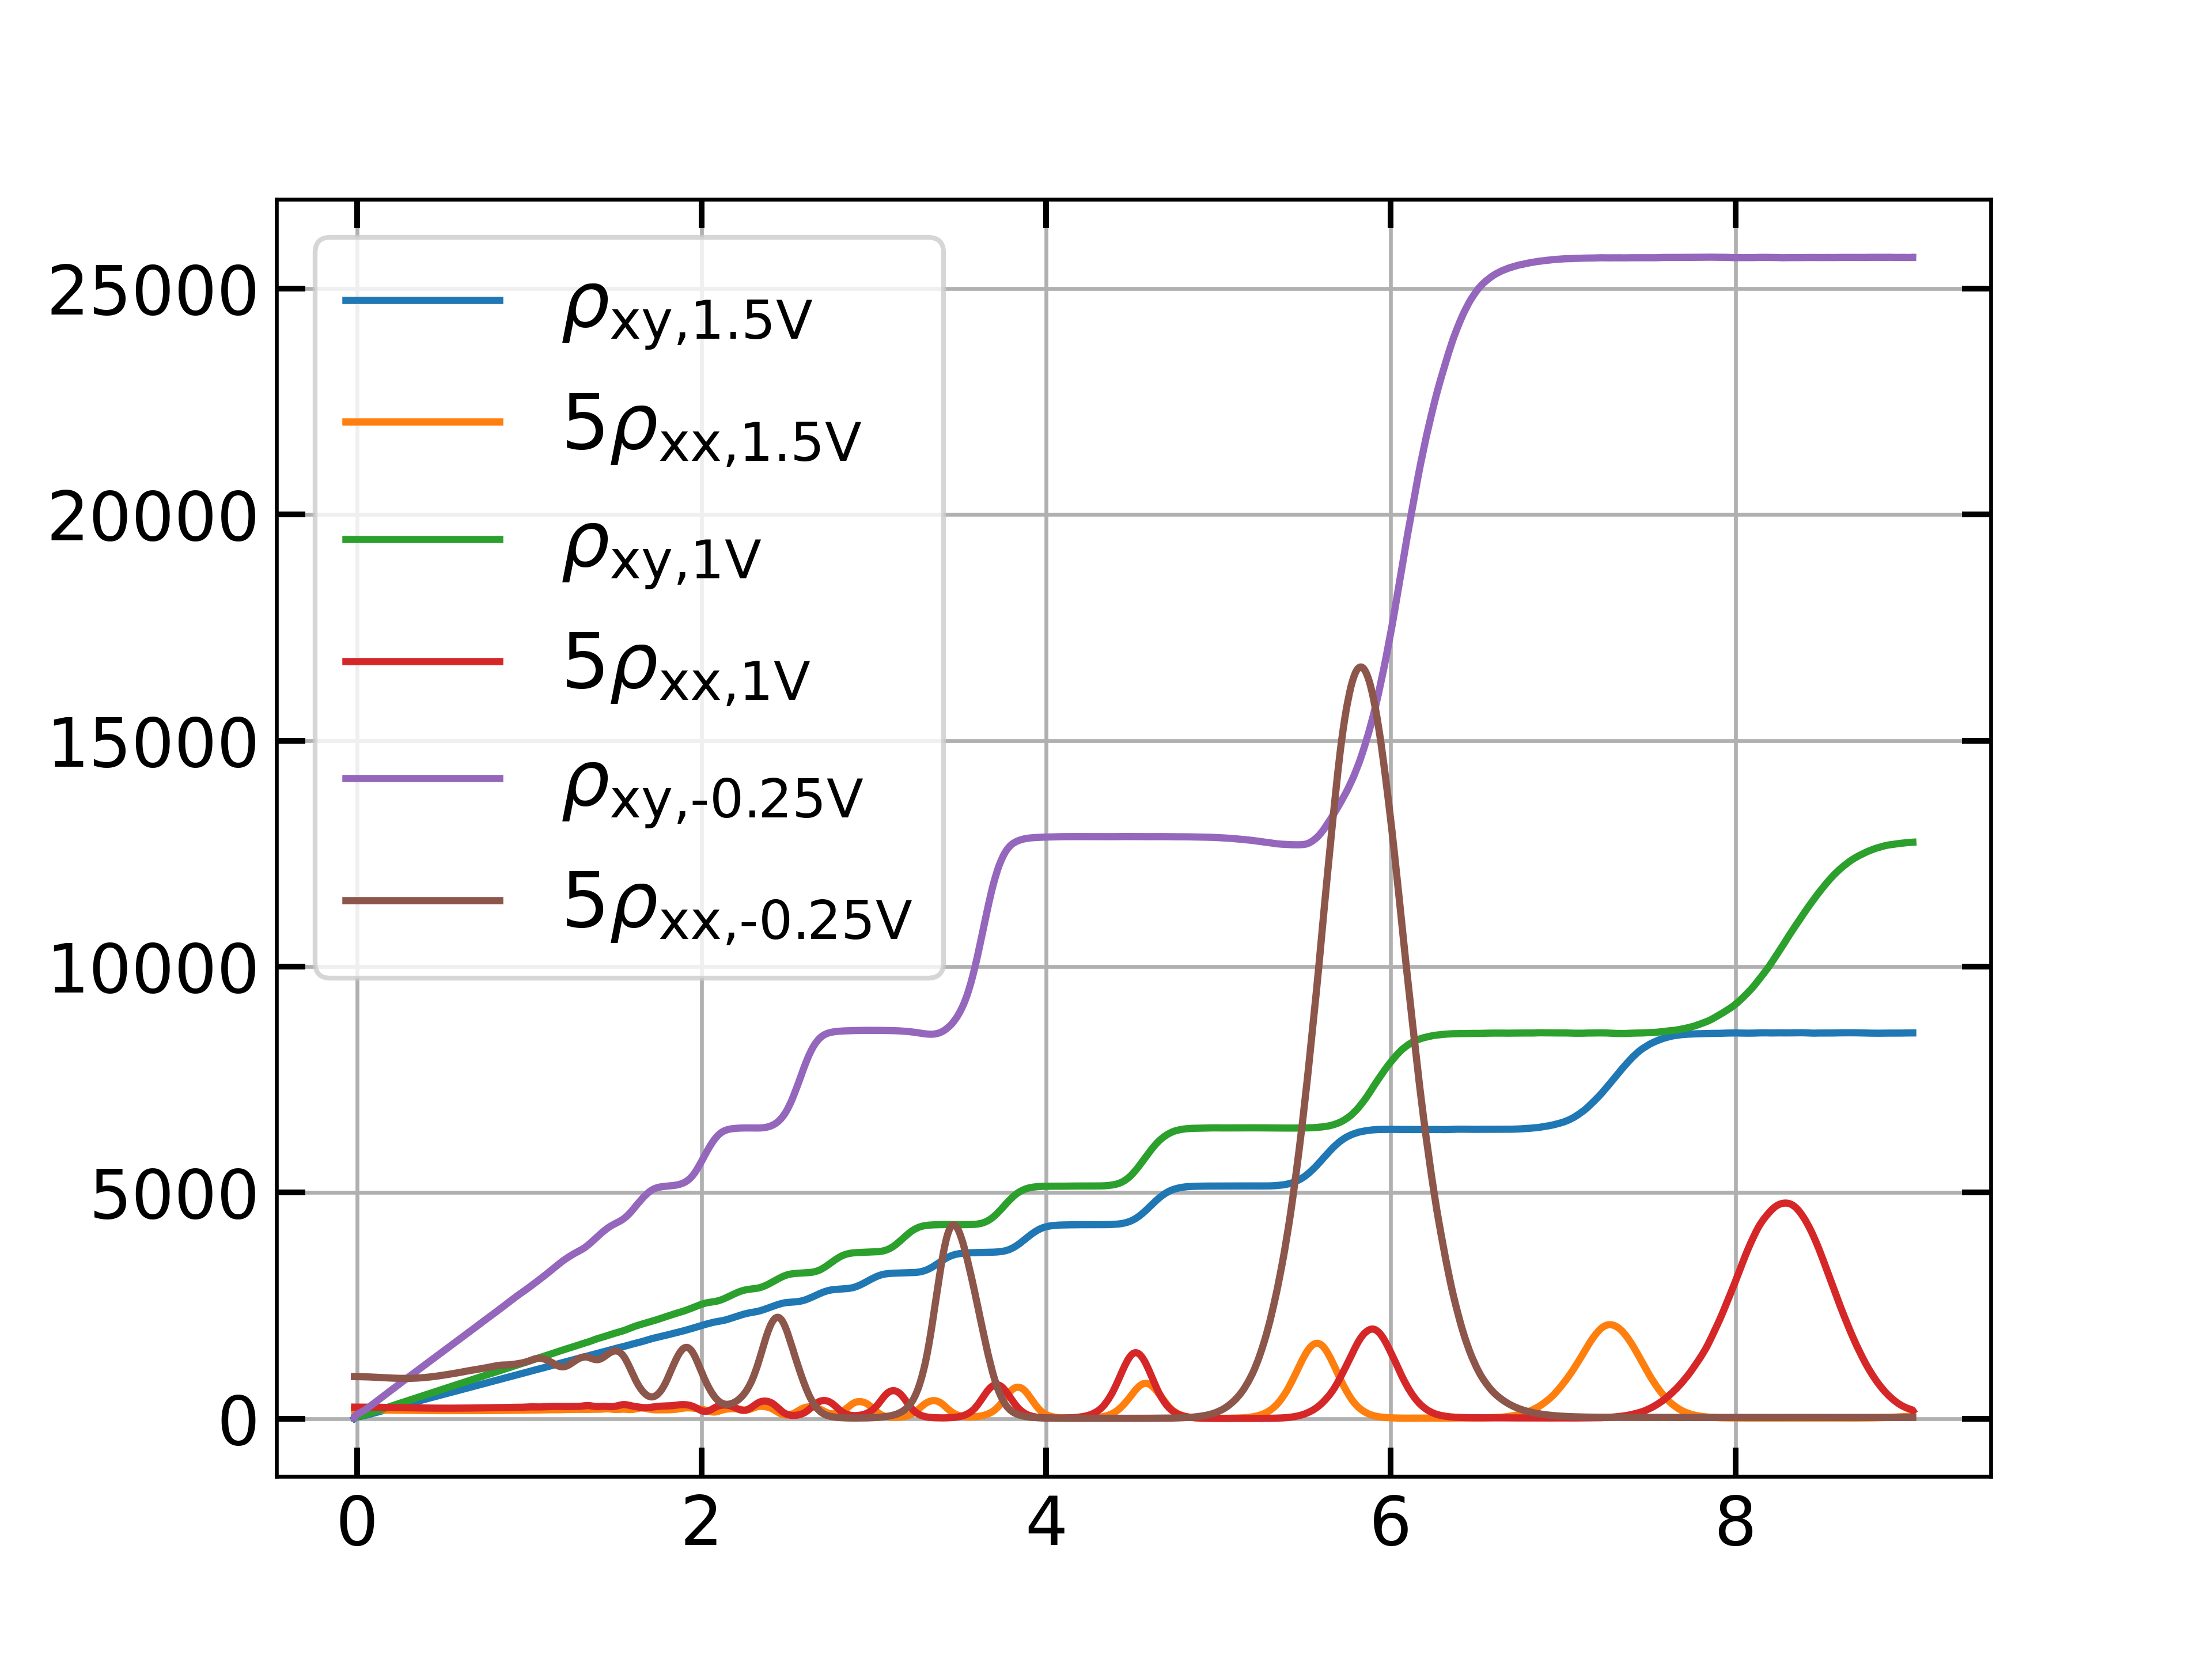
\includegraphics[width=0.45\textwidth]{../Images/differentGateVoltagesQHE.png}
    \caption{Resistivities $\rho_\text{xy}$ and $\rho_\text{xx}$ for different gate voltages at $1.4K$. 
    All 6 curves are in the regime of electron conduction.
    Lower $U_\text{gate}$
     leads to a steeper incline of $\rho_\text{xy}$ and higher peaks in $\rho_\text{xx}$ with larger gaps in between.
    The plateaus keep their discrete values.
}
    \label{fig:differentGateVoltagesQHE}
\end{figure}
In these three cases, the Fermi level remains above (or at, for $\nu=1$) the lowest Landau level.
Note that for fixed $n$ the lowest Landau level will not cross the Fermi level by increasing $B$.
However, the Fermi level can be shifted below the lowest Landau level if $U_\text{gate}$ and the corresponding $n$ are low enough.
Then only niveaus corresponding to defects will be around the Fermi level.
If $U_\text{gate}$ is lowered further, the Fermi level will cross the band gap from the conduction band to the valence band.
More Landau niveaus should appear, but the corresponding charge carriers are no longer electrons, but holes.
This effect is investigated with $U_\text{gate}=-1V,\,-1.5V$.
The resistances for these gate voltages are plotted in \ref{fig:kaputteKurvenGateV}.
\begin{figure}[h]
    \centering
    
\includegraphics[width=0.45\textwidth]{../Images/kaputteKurvenGateV.png}
    \caption{
        Resistances $\rho_\text{xy}$ and $\rho_\text{xx}$ at $1.4K$ for different gate voltages, corresponding to low carrier densities $n$.  
        The slope for small $B$ indicates the small value of $n$.
        Defects may play an important role for small $n$.
        Negative $\rho_\text{xy}$ correspond to p-type conduction, positive $\rho_\text{xy}$ to n-type conduction.}
    \label{fig:kaputteKurvenGateV}
\end{figure}
For the gate voltage of $1V$ the carrier density is very low, resulting in the steep slope of $\rho_\text{xy}$.
This explains why the plateau corresponding to $\nu=1$ is already reached at $B\approx1.6T$ and the plateaus corresponding to $\nu\>1$ are not visible.
The longitudinal component has vanishing resistivity for values of $B$ where $\rho_\text{xy}$ is constant.
For these small carrier densities, defects with localized states could play an increasingly important role.
After further increasing $B$, $\rho_\text{xy}$ temporarily shows negative values.
This could be explained by p-type conduction, since the holes with positive charges moving in the opposite direction are deflected in the same direction as the electrons, resulting in a sign change of $\rho_\text{xy}$.
Since the valence band typically has a smaller curvature near the band gap, the holes typically have a larger effective mass $m^\star$.
The cyclotron frequency
\begin{align}
    \omega_c = \frac{eB}{m^\star}    
\end{align}
an therefore the energy (difference) of the Laudau levels
\begin{align}
    \epsilon = \hbar \omega_c \left(\frac{1}{2} + n_\text L \right)
\end{align}
is smaller for the holes.
This makes the Landau levels more difficult to separate. 
Larger $B$ would be needed to get the same results as with electrons.
The $\rho_\text{xy}$ of $U_\text{gate} = -1.5V$ has a negative slope for small $B$.
This is interpreted as p-type conduction, resulting in a negative carrier density.
Note that the transverse conductivity does not vanish for $B=0$.
This could be a sign of anisotropy in the material.
It is unclear why this shift only applies to holes.
$\rho_\text{xy}$ for $U_\text{gate} = -1.5V$ does not reach the von Klitzing constant.
It is assumed that even smaller $U_\text{gate}$ will show plateaus.

Extrapolating $n$ for lower $U_\text{gate}$ gives an estimate for the charge carrier density (see fig. \ref{fig:extrapolating})
\begin{figure}[h]
    \centering
    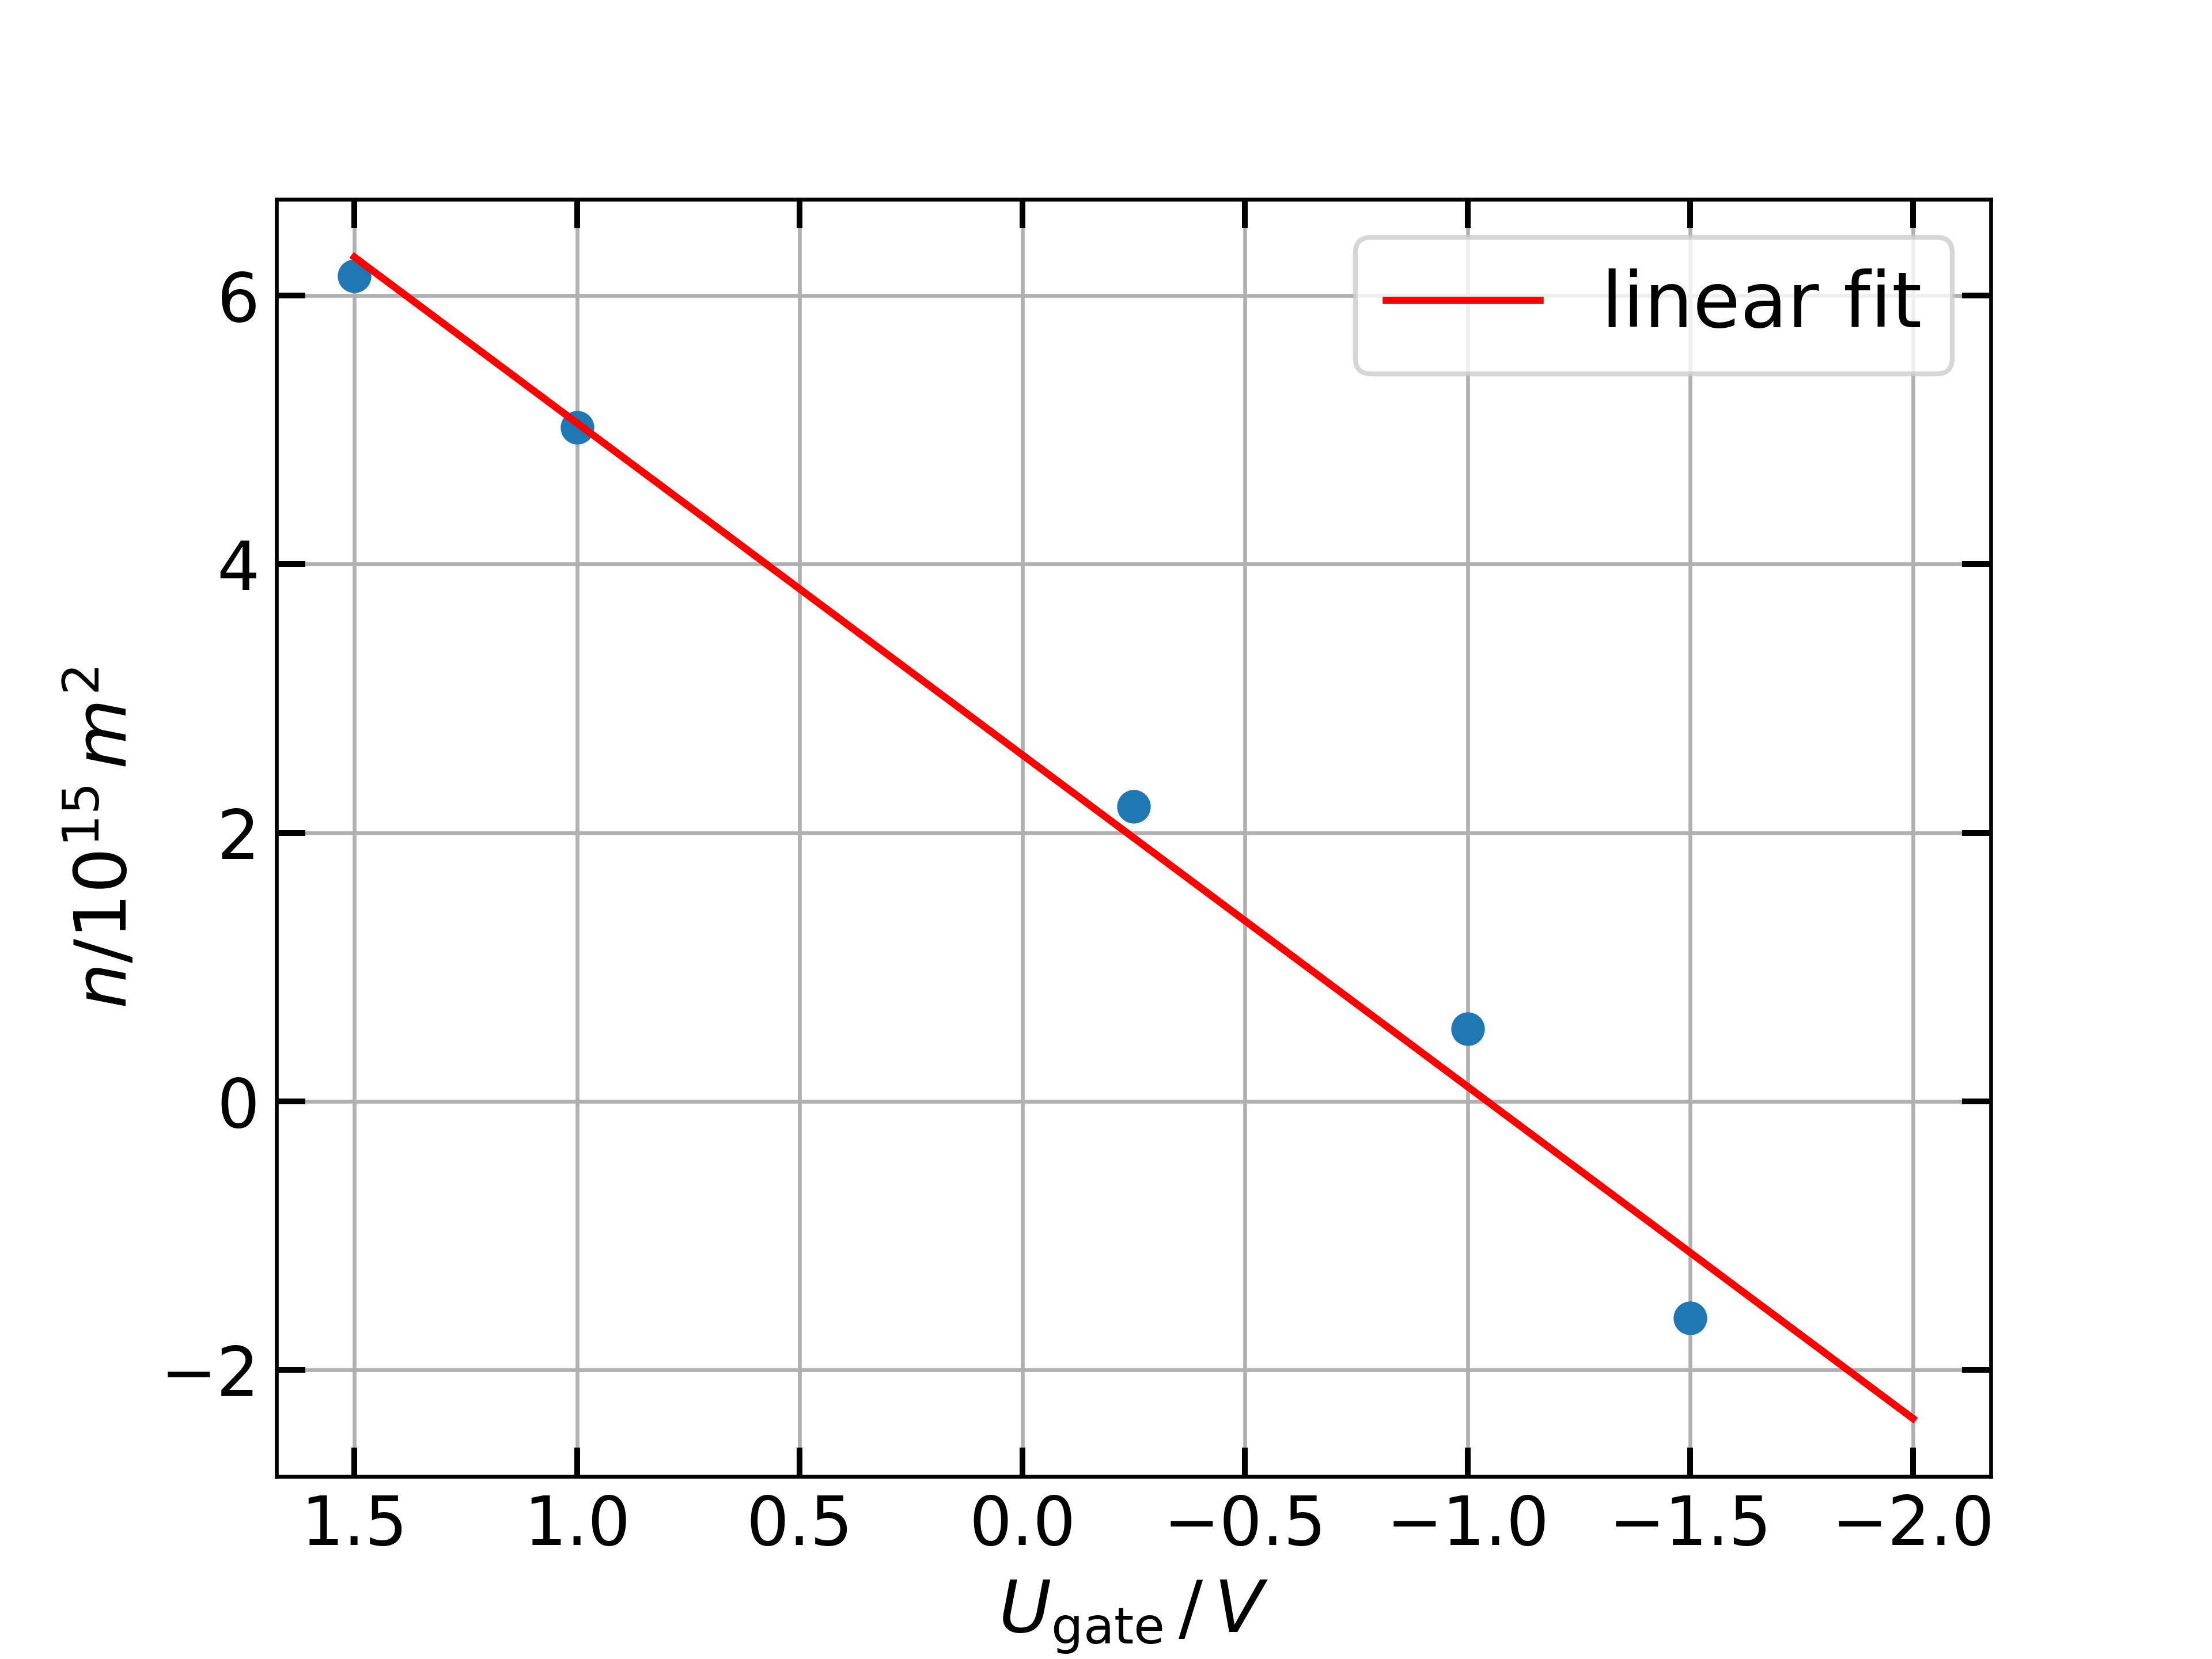
\includegraphics[width=0.45\textwidth]{../Images/extrapolatingN.png}
    \caption{
        Dependence of charge carrier density $n$ on gate voltage.
        The linear fit is extrapolated to estimate the gate voltage required to have a hole carrier density comparable to the electron carrier density with $U_\text{gate} = -0.25\,\text{V}$.}
    \label{fig:extrapolating}
\end{figure}
To obtain a hole carrier density comparable to the electron carrier density for $U_\text{gate} = -0.25\,\text{V}$,
a gate voltage of $U_\text{gate} \approx -2\,V$ is required.
